\documentclass[t]{beamer}
\usepackage[utf8x]{inputenc}
\usepackage[ngerman]{babel}
\usepackage[T1]{fontenc}
\usepackage{textcomp}
\usepackage{subfigure}
\usepackage{graphicx}
\usepackage{fancyhdr}
\usepackage{tgpagella}
\usepackage[absolute,overlay]{textpos}
\usepackage{hyperref}
\usepackage{wasysym}
% \MakeAutoQuote{„}{”}

% ohne dieses Paket bekommt Carsten verpixelte Schrifen
\usepackage{lmodern}

\hypersetup{
colorlinks=true,
linkcolor=[rgb]{1, 1, 1}, %
urlcolor=[rgb]{.2, .2, .5} %
%allcolors=[rgb]{0, 0, 0} % schwarz
}

\usetheme{Dresden}
\setbeamertemplate{navigation symbols}{} % we dont want navigation buttons

\title{Freie Software Freies Wissen Dresden}
\subtitle{UniStick-Ausgabe-Veranstaltung}
\author{\texttt{https://fsfw-dresden.de}}
\date{17. Oktober 2016}



\addtobeamertemplate{frametitle}{}{%
  \begin{textblock*}{130mm}(.963\textwidth,8.4mm)
    \includegraphics[width=2.25cm]{img-src/fsfw-logo.pdf}
  \end{textblock*}
}


\setbeamercolor{frametitle}{fg=black}

\synctex=1

% \includeonlyframes{p1}

\begin{document}









%  Feedback 1
% >
% > Spät, aber ich habe noch ein paar Anmerkungen zum Vortrag: Ich hätte erst
% > kurz(!) gesagt was Freie Software eigentlich heißt bevor du versuchst zu
% > erklären warum das Toll ist. Ich glaube das hilft dabei zu verstehen was
% > überhaupt passiert. Vielleicht einfach die "vier Freiheiten" vor "Warum machen
% > wir das?" ziehen.
% >
% > Ich hätte außerdem nicht die ganze Zeit gesagt, dass es kurz gehalten wird --
% > das wirkt irgendwie unprofessionell.
% >
% > Vom Siezen war ich auch nicht überzeugt, so von Hochschulgruppe zu Studenten
% > wirkt mir das zu distanziert irgendwie.


% Feedback 2: lieber Windows und libre Office zeigen, als Linux und LaTeX
% (verstehe ich, aber überzeugt mich nicht hinreichend)


\begin{frame}[label=p1]
  \begin{center}%
\vspace*{-1em}
\includegraphics[width=4cm]{img-src/fsfw-logo-with-text}
\hspace{1cm}
\includegraphics[width=4cm]{img-src/gutschein-seite-1}\\
\vspace{1em}
\structure{\Large "`UniStick-Ausgabe-Veranstaltung"'}
  \end{center}
\end{frame}

%%%%%%%%%%%%%%%%%%%%%%%%%%%%%%%%%%%%%%%%%%%%%%%%%%%%%%%%%%%%%%%%%%%%%%%%%%%%%%%%

\begin{frame}[label=ol]{\usebeamercolor[fg]{structure}\color{fg}Überblick}
  \begin{itemize}
  \item Wer sind wir?
  \item Was kann der Stick?
  \item Verteilung der Sticks
  \end{itemize}
\end{frame}

%%%%%%%%%%%%%%%%%%%%%%%%%%%%%%%%%%%%%%%%%%%%%%%%%%%%%%%%%%%%%%%%%%%%%%%%%%%%%%%%

\begin{frame}[label=photo,plain]{\usebeamercolor[fg]{structure}\color{fg}Fotos? (Persönlichkeitsrechte)}
\vspace{10mm}
\begin{center}
\includegraphics[width=0.8\textwidth]{img-src/annonymitaet}

\end{center}

\end{frame}


%%%%%%%%%%%%%%%%%%%%%%%%%%%%%%%%%%%%%%%%%%%%%%%%%%%%%%%%%%%%%%%%%%%%%%%%%%%%%%%%

\begin{frame}[label=ct1]{\usebeamercolor[fg]{structure}\color{fg}FSFW (1)}
Wer sind wir?
  \begin{itemize}
  \item Hochschulgruppe (gegründet 2014, ca. 10 P.)
  \item bisherige Projekte:
  \begin{itemize}
   \item Linux-Install-Party, Linux-Presentation-Day
   \item Verschlüsselungsgewinnspiel
   \item Monatliche \href{https://fsfw-dresden.de/sprechstunde}{Sprechstunde} (Textsatzsystem \LaTeX, UniStick, ...)
   \item Publikationen: \href{https://fsfw-dresden.de/programm}{Programmpapier}, \href{https://fsfw-dresden.de/blog}{Blogbeiträge}
   \item Workshops (\href{https://fsfw-dresden.de/git-ws}{git}, \href{https://fsfw-dresden.de/python-workshop}{python},
   \href{https://fsfw-dresden.de/gpg}{Mailverschlüsselung})
   \item Ringvorlesung: "`\href{https://fsfw-dresden.de/ringvorlesung}{Freie Software und Freies Wissen als Beruf}"'
   \smallskip
   \item UniStick mit freier Software
  \end{itemize}
  \end{itemize}
\end{frame}

%%%%%%%%%%%%%%%%%%%%%%%%%%%%%%%%%%%%%%%%%%%%%%%%%%%%%%%%%%%%%%%%%%%%%%%%%%%%%%%%

\begin{frame}[label=ct2]{\usebeamercolor[fg]{structure}\color{fg}FSFW (2)}
Warum machen wir das? $\rightarrow$ \textbf{Aus Überzeugung}\\[1cm]
  \begin{itemize}
  \item Überzeugung 1: freie und quelloffene Software ist (meist) besser
  \item[] technische/nicht technische Argumente
  \pause
  \bigskip
  \item Überzeugung 2: \textit{öffentlich finanzierte} wissenschaftliche Inhalte
  (AutorInnen, GutachterInnen) sollten nicht von \textit{öffentlich finanzierten}
  Bibliotheken für \textit{horrende Summen} von Zeitschriften-Verlagen gekauft werden müssen
  \end{itemize}
\end{frame}

%%%%%%%%%%%%%%%%%%%%%%%%%%%%%%%%%%%%%%%%%%%%%%%%%%%%%%%%%%%%%%%%%%%%%%%%%%%%%%%%

\begin{frame}[label=ct3,plain]{}

\vspace{1mm}
\begin{center}
\includegraphics[width=1.05\textwidth]{img-src/tud-ich-muss-etwas-tun}
\end{center}


\end{frame}


%%%%%%%%%%%%%%%%%%%%%%%%%%%%%%%%%%%%%%%%%%%%%%%%%%%%%%%%%%%%%%%%%%%%%%%%%%%%%%%%
\begin{frame}[label=wb]{\usebeamercolor[fg]{structure}\color{fg}Software: Frei versus Proprietär}

\begin{columns}

\column[t]{0.02\textwidth}

~
\column[t]{0.5\textwidth}
Vier Freiheiten freier Software\\[4mm]
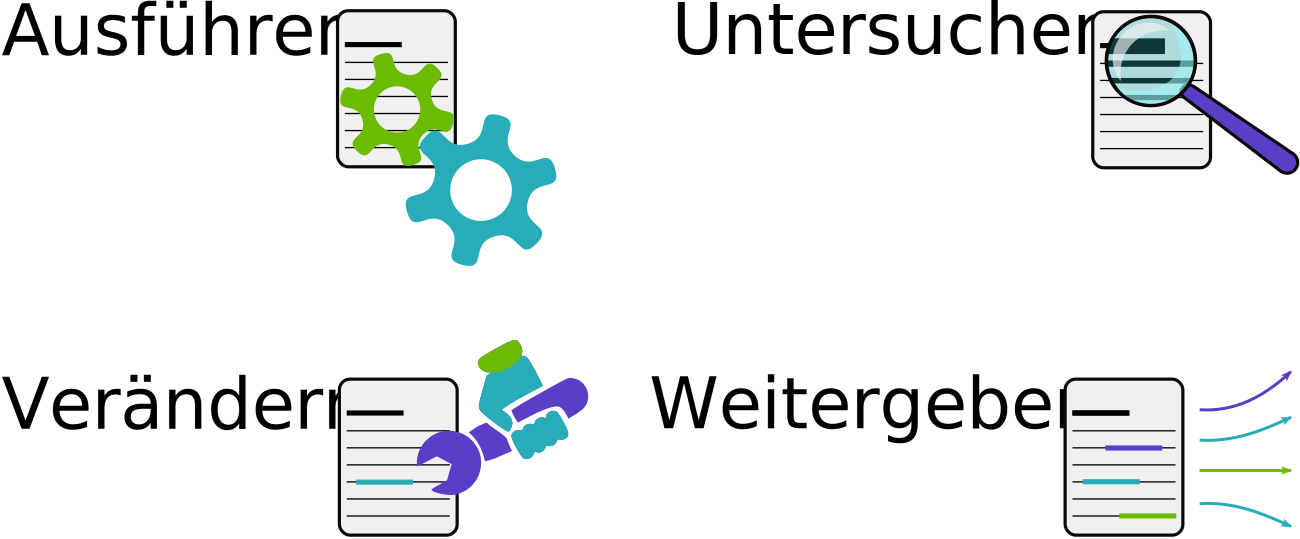
\includegraphics[width=40mm]{img-src/vier-freiheiten}
\pause

Vorteile:
\begin{itemize}
\item Kontrolle behalten
\item Erkenntnisgewinn
\item Lizenzkosten: 0 €
\item Anpassbarkeit an eigene Bedürfnisse
\item Hersteller-Unabhängigkeit\\[-2mm] {\tiny (kein Vendor Lock-in)}

\end{itemize}


\column[t]{0.01\textwidth}
~
\column[t]{0.58\textwidth}
Nachteile Proprietärer Software
\begin{itemize}
 \item Intransparenz {\tiny (Bsp: Wahlsoftware)}
 \item Hintertüren? {\tiny (Win10-Verbot für Dienstgebrauch)}
 \item Abhängigkeit
\end{itemize}
 \pause
 \bigskip


 \textit{Warum gibt es MS-Office eigentlich {\color<4->{red} \visible<4->{"`}kostenlos\visible<4->{"'}} für Studierende?}

 \pause
 \pause
 \medskip
 \rule{\textwidth}{1pt}\\[2mm]
%  \smallskip
 Offener Brief:\\

 "`public money $\Rightarrow$ public code"'\\[2mm]

 \url{https://publiccode.eu}


\end{columns}

\end{frame}

%%%%%%%%%%%%%%%%%%%%%%%%%%%%%%%%%%%%%%%%%%%%%%%%%%%%%%%%%%%%%%%%%%%%%%%%%%%%%%%%
\begin{frame}[label=ct4]{\usebeamercolor[fg]{structure}\color{fg}Freie Software an der TU (1) }

\begin{itemize}
 \item ZIH: Es gibt eine \href{https://tu-dresden.de/zih/dienste/software-auswahl-und-open-source-strategie}{Open-Source-Strategie}
 \item StuRa: Bietet viele \href{https://wiki.stura.tu-dresden.de/doku.php?id=allgemein:dienste:start}{digitale Dienste} auf Basis freier Software
\begin{itemize}
 \item Mumble (Telefonkonferenzen)
 \item Kanban (Gruppenorganisation)
 \item Etherpad (gemeinsam Texte schreiben)
 \item ...

\end{itemize}

\end{itemize}

\end{frame}

%%%%%%%%%%%%%%%%%%%%%%%%%%%%%%%%%%%%%%%%%%%%%%%%%%%%%%%%%%%%%%%%%%%%%%%%%%%%%%%%

\begin{frame}[t,label=ct5]{\usebeamercolor[fg]{structure}\color{fg}Freie Software an der TU (2)}

\vspace{-5mm}

\begin{columns}
\column[t]{0.5\textwidth}

\vspace{-4mm}
\begin{center}
\href{https://fsfw-dresden.de/ringvorlesung}{\includegraphics[width=50mm]{img-src/FSFW-RV}}
\end{center}

\column[t]{0.5\textwidth}

  Ringvorlesung im WiSe 18/19
  \medskip

  \begin{center}
  \textit{Freie Software und Freies Wissen als Beruf}
  \end{center}

  \smallskip

  \begin{itemize}
   \item[$\rightarrow$] interessant
   \item[$\rightarrow$] bis zu 3 CP (AQUA)
  \end{itemize}

  \bigskip
  Zeit: Dienstags, 17-18:30 Uhr

  \smallskip
  Ort: HTW Dresden, Raum Z 254

  \bigskip
  Infos: {\scriptsize \url{fsfw-dresden.de/ringvorlesung}}

\end{columns}

\end{frame}

%%%%%%%%%%%%%%%%%%%%%%%%%%%%%%%%%%%%%%%%%%%%%%%%%%%%%%%%%%%%%%%%%%%%%%%%%%%%%%%%

\begin{frame}[label=vf1]{\usebeamercolor[fg]{structure}\color{fg}Vorführung des Sticks}
Struktur: Linux-Live-System (Debian stable ) + Windows-Partition\\[3mm]

\textbf{Was ist ein Live-System?}
\begin{itemize}
  \item Betriebssystem, das von USB-Stick bootet
  \item[]
  \item Keine Änderungen am eigenen PC
  \item[$\rightarrow$] Unkompliziertes Ausprobieren
  \item[]
  \end{itemize}

\pause
\textbf{Was haben wir gemacht?}
  \begin{itemize}
  \item Auswahl von Software (Zielgruppe Studierende)
  \item insb. auch Anwendungen die ohne Installation auskommen
  \item Dokumentation $\rightarrow$ \texttt{FSFW-Material}
  \item Konfiguration
  \end{itemize}

\end{frame}



%%%%%%%%%%%%%%%%%%%%%%%%%%%%%%%%%%%%%%%%%%%%%%%%%%%%%%%%%%%%%%%%%%%%%%%%%%%%%%%%

\begin{frame}[label=ct4]{\usebeamercolor[fg]{structure}\color{fg}{}}
 \vspace{20mm}

\begin{center}
Vorführung\\ ... \\[10mm]

{\tiny (Anhand der \href{https://github.com/fsfw-dresden/usb-live-linux/blob/master/doc/src/index.md}{Dokumentation})}



\end{center}
\end{frame}

%%%%%%%%%%%%%%%%%%%%%%%%%%%%%%%%%%%%%%%%%%%%%%%%%%%%%%%%%%%%%%%%%%%%%%%%%%%%%%%%

\begin{frame}[label=ct5]{\usebeamercolor[fg]{structure}\color{fg}{Weitere Informationen}}
 \vspace{6mm}
 Fehlerkorrekturen, Anleitungen etc.
 \vspace{6mm}

% \begin{center}
\url{https://fsfw-dresden.de/uni-stick} {\tiny(siehe Gutschein)}\\[3mm]

\url{https://fsfw-dresden.de/sprechstunde} {\tiny(Dienstags, 19:30 Uhr)}\\[3mm]
\url{https://fsfw-dresden.de/newsletter} {\tiny (kommt selten, sehr informativ)}\\[3mm]

\url{https://fsfw-dresden.de/mitmachen} {\tiny(Plenum: Do. (ungerade KW))}\\[3mm]

\url{kontakt@fsfw-dresden.de} \\[3mm]




% \end{center}
\end{frame}


%%%%%%%%%%%%%%%%%%%%%%%%%%%%%%%%%%%%%%%%%%%%%%%%%%%%%%%%%%%%%%%%%%%%%%%%%%%%%%%%

% \begin{frame}[label=ct6]{\usebeamercolor[fg]{structure}\color{fg}{Anschlusskommunikation (1)}}
%
%
%  \begin{center}
%
%  \includegraphics[width=4cm]{img-src/datenspuren}
%   \end{center}
%
%
%   "`Datenspuren"'
%   \begin{itemize}
%    \item Symposium des \textbf{C}haos \textbf{C}omputer \textbf{C}lub \textbf{D}res\textbf{d}en
%    \item 21. \& 22. Okt. \pause technische Sammlungen
%    \item Vorträge, Stände, ...
%    \smallskip
%    \item \url{https://www.datenspuren.de/2017/}
%
%   \end{itemize}
%
%
% %   \pause
%
% \begin{textblock*}{10mm}[0.,0.](97mm, 55mm)
% \visible<2->{
% \includegraphics[width=25mm]{img-src/technische-sammlungen}
% }
% \end{textblock*}
%
%
%
% \end{frame}



%%%%%%%%%%%%%%%%%%%%%%%%%%%%%%%%%%%%%%%%%%%%%%%%%%%%%%%%%%%%%%%%%%%%%%%%%%%%%%%%

\begin{frame}[label=ct8]{\usebeamercolor[fg]{structure}\color{fg}{Verteilung der Sticks}}
 \vspace{10mm}
Zwei Möglichkeiten:\\[10mm]
\begin{center}
"`Bürokratie"'  \qquad versus \qquad "`Tumult"'
\end{center}
\end{frame}

%%%%%%%%%%%%%%%%%%%%%%%%%%%%%%%%%%%%%%%%%%%%%%%%%%%%%%%%%%%%%%%%%%%%%%%%%%%%%%%%





% \begin{frame}[label=ol]{\usebeamercolor[fg]{structure}\color{fg}Metadaten}
%     \begin{itemize}
%     \item Mit Mitgliedern von der HTW (andere Unis pending)
%     \end{itemize}
%   \item Insb. kein Verein: Nutzen der Hochschulresourcen, Hochschule als Zielgruppe und Arbeitsfeld.
%   \end{itemize}
% \end{frame}
%
% \begin{frame}{\usebeamercolor[fg]{structure}\color{fg}Arbeitsthesen}
%   \begin{itemize}
%   \item<1-> Freie Software und freies Wissen fördert die Bildung einer aufgeklärten digitalen Gesellschaft
%   \item<2-> Freie Software fördert Wahlfreiheit und schützt vor Abhängigkeit
%   \item<3-> Freie Software erhöht Nachvollziehbarkeit
%   \item<4-> Freie Lizenzen sichern den ungehinderten Zugang zu öffentlich finanzierter Forschung
%   \end{itemize}
% \end{frame}
%
% \begin{frame}{\usebeamercolor[fg]{structure}\color{fg}Interesse?}
%   \begin{description}
%   \item[Web] \url{https://fsfw-dresden.de}\\
%     \includegraphics[width=4cm]{img-src/website-qr.pdf}
%   \item[Mailingliste] \url{https://lists.fsfw-dresden.de/mailman/listinfo/discuss} (auch oben verlinkt)
%   \item[Treffen] SLUB (Hauptgebäude), Raum -2.115, Donnerstags in ungeraden Wochen, 18:30 Uhr
%   \end{description}
% \end{frame}

\end{document}
